\chapter{Relations et opérations fondamentales dans l'ensemble des nombres décimaux et des fractions}
%\stepcounter{module}
 
{\AlegreyaSansLight \large
\begin{center}
\textbf{Crédit :} 32 heures\\
\textit{4 heures hebdomadaires}
\end{center}
}

\minitoc

\section{Introduction}
\subsection{Présentation du module}
Ce module vise à rendre l'apprenant compétent dans des situations de vie de la famille « \textit{représentation, détermination des quantités et identification des objets
par des nombres} ». Il s'agit en gros, de le rendre capable de :
\begin{itemize}
\item Résoudre des problèmes relatifs à des situations de vie telles que : l'achat ou la vente des biens de consommation, le partage des biens, la vérification
d'une facture après payement, la comparaison des prix des objets …
\item Communiquer des informations comportant des nombres (numéros de téléphones, matricule, immatriculation d'un véhicule …).
\end{itemize}
Il importe pour cela de consolider les notions d'addition, de soustraction, de multiplication, de division et de relation d'ordre vues dans le cycle primaire avec
cependant une démarcation significative dans l'introduction et la manipulation des nombres décimaux relatifs, sur lesquels l'utilisateur devrait s'appesantir un peu plus.
On restera au niveau des habiletés cognitives que sont : la connaissance et la compréhension.\\
En dehors de la maîtrise des techniques opératoires, il est question de donner du sens aux nombres décimaux et de les utiliser dans des situations de vie qui l'exigent.

\subsection{Contribution du module à la finalité et aux buts curriculaires}
Ce module permet de développer le sens de l'ordre, de la concision et l'esprit critique. Il contribue au renforcement de la pratique du calcul mental ou à l'utilisation de la calculatrice, ce qui permet à l'apprenant d'agir de manière autonome, compétente et adaptative dans diverses situations de la vie courante, dans lesquelles ces pratiques interviennent.

\subsection{Contribution du module au programme d'études et aux domaines de vie}
Ce module qui fait partie des programmes de mathématiques permet à chaque apprenant d'acquérir des connaissances et savoir-faire de base sur lesquels les
enseignements/apprentissages qu'il recevra ultérieurement dans les autres disciplines du domaine d'apprentissage devront s'appuyer. Les nombres décimaux sont
utilisés dans toutes les sciences pour mesurer, peser et évaluer les quantités.\\
La maîtrise des concepts d'égalité, d'inégalité et des opérations fondamentales que sont l'addition, la soustraction, la multiplication et la division, est de nature à
doter l'apprenant d'un des outils fondamentaux dont il aura besoin tout au long de sa vie. La gestion du budget familial, la comptabilité au sein de l'entreprise,
l'évaluation des distances, des poids, des aires et des volumes, sont autant d'applications des nombres décimaux dans les domaines de vie que sont l'économie, les
média, l'environnement, la santé et le bien être.

\section{Matrice}


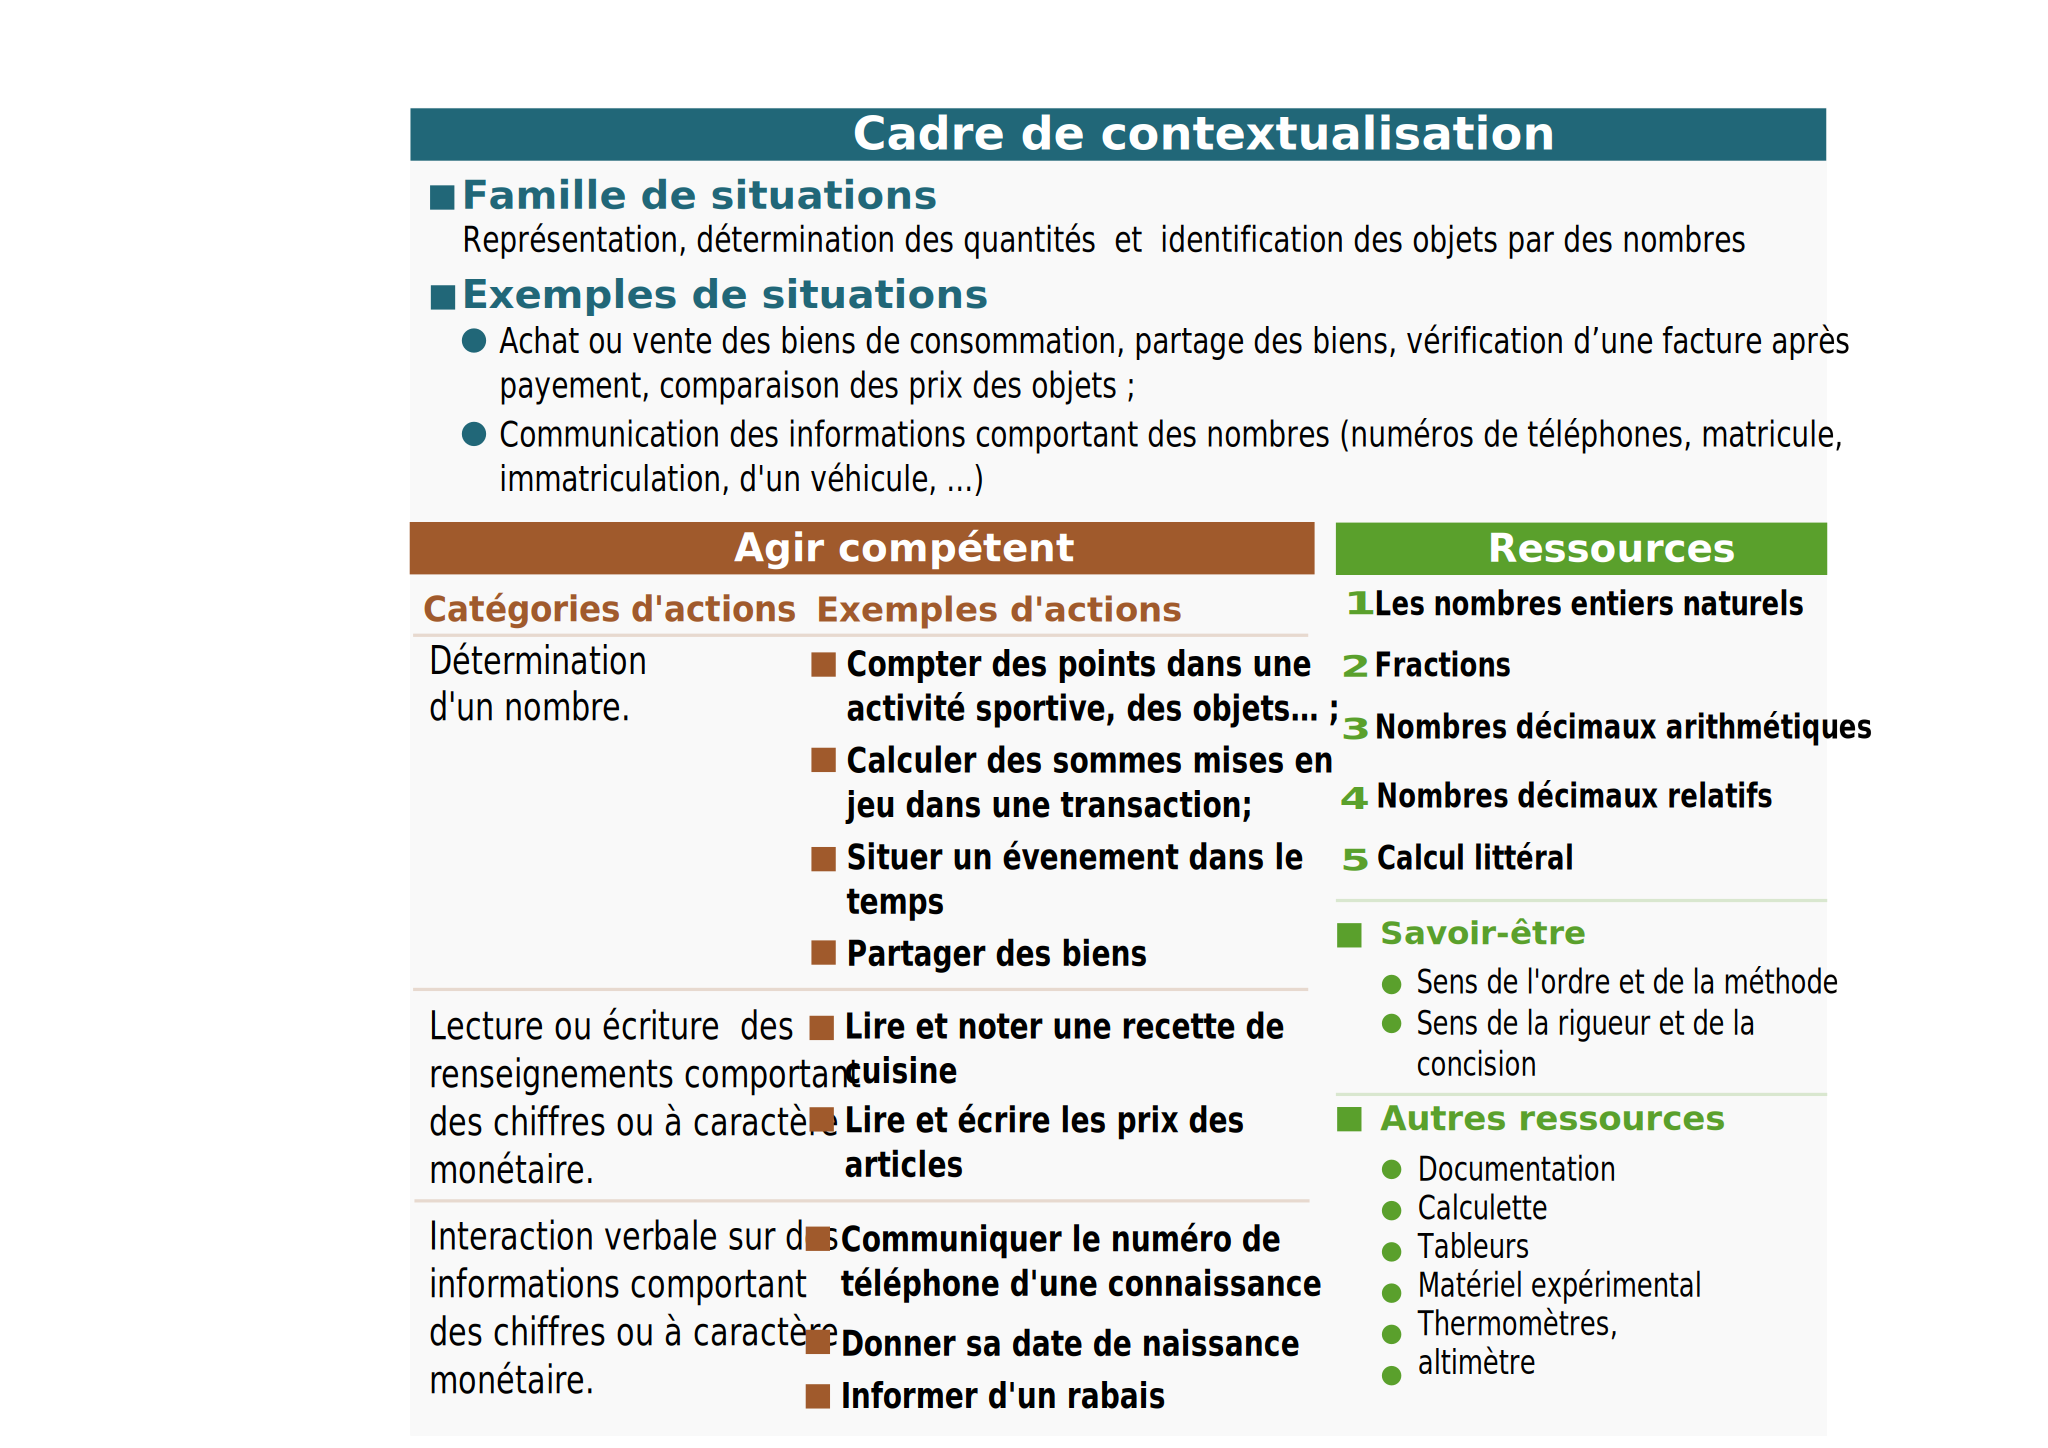
\includegraphics[width=\textwidth]{Module1.pdf} 

\subsection*{}
\addcontentsline{toc}{subsection}{\textbf{Ressource 1}: Les nombres entiers naturels}
\ressource{IN.pdf}

\savoir
\begin{itemize}
\item Multiples et diviseurs d'un entier naturel.
\item Entiers naturels et ordre ;
\item Entiers naturels consécutifs ;
\item Propriétés d'addition et de multiplication des nombres entiers naturels.
\end{itemize}
\savoirfaire
\begin{itemize}
\item Lecture et écriture des entiers;
\item Opérations d'addition, de soustraction, de multiplication et de division;
\item Division à l'aide des critères de divisibilité : par 10, 100, 1000, .., par 2 , 3, 5 et  9;
\item Nombre d'entiers consécutifs de m à n où n et m sont des entiers naturels.
\end{itemize}

\subsection*{}
\addcontentsline{toc}{subsection}{\textbf{Ressource 2}: Les fractions}
\ressource{Fractions.pdf}

\savoir
\begin{itemize}
\item Numérateur, dénominateur, fractions égales, fractions irréductibles, fractions décimales ;
\item Inverse d'une fraction;
\item Propriétés d'addition et de multiplication des fractions.
\end{itemize}
\savoirfaire
\begin{itemize}
\item Ecriture fractionnaire d'un nombre décimal;
\item Simplification des fractions;
\item Addition et soustraction des fractions de même dénominateur;
\item Multiplication, division des fractions;
\item Comparaison des fractions.
\end{itemize}

\subsection*{}
\addcontentsline{toc}{subsection}{\textbf{Ressource 3}: Nombres décimaux arithmétiques}
\ressource{ID.pdf}

\savoir
\begin{itemize}
\item Lecture et écriture d'un nombre décimal;
\item Propriétés d'addition et de multiplication des nombres décimaux.
\end{itemize}
\savoirfaire

\textbf{Techniques et méthodes}
\begin{itemize}
\item \textit{Opérations} : addition, soustraction, multiplication, division ;
\item Comparaison des nombres décimaux..
\end{itemize}

\subsection*{}
\addcontentsline{toc}{subsection}{\textbf{Ressource 4}: Nombres décimaux relatifs}
\ressource{Z.pdf}

\savoir
\begin{itemize}
\item Nombres entiers relatifs;
\item Opposé d'un nombre décimal relatif.
\end{itemize}
\savoirfaire
\begin{itemize}
\item Somme d'entiers relatifs;
\item Somme de décimaux relatifs.
\end{itemize}

\subsection*{}
\addcontentsline{toc}{subsection}{\textbf{Ressource 5}: Calcul littéral}
\ressource{CL.pdf}

\savoir

\textbf{Règles de priorité des opérations :}
\begin{itemize}
\item opérations avec parenthèses ;
\item opérations sans parenthèses ;
\item suite de multiplications et de divisions sans parenthèses.
\end{itemize}
\savoirfaire
\begin{itemize}
\item Valeur numérique d'une expression littérale simple ;
\item Utilisation des propriétés de l'addition et de la multiplication des nombres décimaux positifs ;
\item Calcul rapide
\end{itemize}